\documentclass[11pt,oneside]{article}

\usepackage[a4paper,margin=27mm,headheight=15pt]{geometry}
\usepackage[T1]{fontenc}
\usepackage[utf8]{inputenc}
\IfFileExists{libertinus.sty}{\usepackage{libertinus}}{\usepackage{lmodern}}
\usepackage{microtype}
\usepackage{amsmath,amssymb,amsthm,mathtools,mathrsfs}
\usepackage{bm}
\usepackage{booktabs,longtable,array,tabularx}
\usepackage{graphicx}
\usepackage{pgfplots}
\usepackage{xcolor}
\usepackage{enumitem}
\usepackage{fancyhdr}
\usepackage{titlesec}
\usepackage{listings}
\usepackage{xurl}
\usepackage{hyperref}
\usepackage[nameinlink,noabbrev]{cleveref}

\definecolor{linkblue}{RGB}{25,75,135}
\definecolor{shadegray}{RGB}{246,247,249}
\definecolor{rulegray}{RGB}{195,201,208}
\pgfplotsset{compat=1.18}
\hypersetup{
  colorlinks=true,
  linkcolor=linkblue,
  citecolor=linkblue,
  urlcolor=linkblue,
  pdftitle={The Decay Envelope of the Rvachev Sinc Product: Second-Wave Audit},
  pdfsubject={Audit of the four synthesis documents; resolution of the unrestricted Cesaro question; corrections to the first audit},
  pdfkeywords={Rvachev up-function, Fabius function, sinc product, Fourier decay, transfer operator, Cesaro mean, Hoischen approximation, law of the iterated logarithm}
}

\pagestyle{fancy}
\fancyhf{}
\fancyhead[L]{\small Fourier-decay audit, second wave}
\fancyhead[R]{\small\nouppercase{\leftmark}}
\fancyfoot[C]{\thepage}
\renewcommand{\headrulewidth}{0.4pt}

\titleformat{\section}{\Large\bfseries}{\thesection}{0.7em}{}
\titleformat{\subsection}{\large\bfseries}{\thesubsection}{0.7em}{}
\titleformat{\subsubsection}{\normalsize\bfseries}{\thesubsubsection}{0.7em}{}
\setcounter{secnumdepth}{3}
\setcounter{tocdepth}{2}
\setlist[itemize]{leftmargin=2em,itemsep=0.25em,topsep=0.4em}
\setlist[enumerate]{leftmargin=2.3em,itemsep=0.25em,topsep=0.4em}
\setlength{\emergencystretch}{2em}
\allowdisplaybreaks

\newtheorem{theorem}{Theorem}[section]
\newtheorem{proposition}[theorem]{Proposition}
\newtheorem{lemma}[theorem]{Lemma}
\newtheorem{corollary}[theorem]{Corollary}
\theoremstyle{definition}
\newtheorem{definition}[theorem]{Definition}
\theoremstyle{remark}
\newtheorem{remark}[theorem]{Remark}
\newtheorem{finding}[theorem]{Finding}
\crefname{finding}{finding}{findings}
\Crefname{finding}{Finding}{Findings}
\newtheorem{erratum}[theorem]{Erratum}
\crefname{erratum}{erratum}{errata}
\Crefname{erratum}{Erratum}{Errata}

\newcommand{\R}{\mathbb R}
\newcommand{\N}{\mathbb N}
\newcommand{\Z}{\mathbb Z}
\newcommand{\Up}{\operatorname{up}}
\newcommand{\sinc}{\operatorname{sinc}}
\newcommand{\e}{\mathrm e}
\newcommand{\dd}{\,\mathrm d}
\newcommand{\Var}{\operatorname{Var}}
\newcommand{\bigO}{\mathcal O}
\newcommand{\vtwo}{v_2}
\newcommand{\T}{T}
\newcommand{\Lop}{\mathcal L}
\newcommand{\Leb}{\operatorname{Leb}}
\newcommand{\lean}[1]{%
  \ifmmode\text{\nolinkurl{#1}}\else\nolinkurl{#1}\fi}

\newenvironment{boxedremark}{%
  \par\smallskip\noindent\begin{center}\begin{minipage}{0.94\textwidth}%
  \color{black}\hrule\vspace{0.6em}\small
}{%
  \vspace{0.6em}\hrule\end{minipage}\end{center}\smallskip
}

\title{\bfseries The Decay Envelope of the Rvachev Sinc Product:\\
Second-Wave Audit\\[0.35em]
\large The unrestricted Ces\`aro question resolved, four syntheses verified,\\
and corrections to the first audit --- including to itself}
\author{Second comparative analysis for Vladimir Reshetnikov's \texttt{ProveIt} project\\
\small covering the four drafts \nolinkurl{rvachev_up_fourier_decay-5} through \nolinkurl{-8}}
\date{27 August 2026}

\begin{document}
\maketitle

\begin{abstract}
Four further documents on the Fourier decay of
$f(x)=\prod_{n\ge0}\sinc(\pi x/2^n)$ arrived after, and in explicit
response to, the comparative audit of the first four
\cite{audit}.  All four are syntheses of the whole corpus, and all four
are essentially correct.  This document audits them, verifies their new
claims, and records what they change.

The mathematical event of the wave is the resolution of the one question
the first audit left open --- and whose answer it guessed wrongly in one
sentence.  Documents~7 and~8 prove, by two independent constructions,
that the \emph{unrestricted} Ces\`aro limit
$\frac1{t-t_0}\int_{t_0}^t|f|/g\to1$ \emph{is} attainable: there exists a
positive, real-analytic, strictly decreasing gauge $g$ with
$\log g(x)=-(\log x)^2/(2\log2)-\kappa_1\log x+o(\log x)$ attaining the
limit for all $t$.  The mechanism --- equalizing the mass of the shell
measures on slowly refining dyadic partitions, hiding the required
upward corrections under the within-shell baseline slope
$-(k+\kappa_1+1)/2$, and finishing with the Hoischen--Carleman theorem
on simultaneous entire approximation of a function and its derivative
--- survives a line-by-line adversarial audit here.  Document~7 also
strengthens the first audit's obstruction from shell-shape-stabilizing
gauges to all bounded-distortion gauges, so the final dichotomy is:
every stabilizing, bounded-distortion, or Hardy-field gauge fails
(Q2); a shell-adaptive analytic gauge with necessarily unbounded,
ever finer within-shell structure attains it.

Document~6 contributes a one-line martingale decomposition
($\mathcal P\psi=\psi/2$, $d=2\psi-\psi\circ T=\log|\tan\pi t|$,
$\int_0^1d^2=\pi^2/4$ exactly) that makes the corrected iterated-logarithm
constant self-contained, and the exact peak-ray identity
$|f(2^n\cdot\tfrac23)|=C_*\,E_{\kappa_\infty}(2^n\cdot\tfrac23)$ for all
$n\ge0$, verified here to $38$ digits with
$C_*=0.13912977473482934529\ldots$  Document~5 sharpens the Gelfond
bound to $\|P_n\|_\infty\le(\sqrt3/2)^{n-1}$ and located the narrow
excursions of the Ces\`aro mantissa profile that the first audit's
$0.025$-step grid missed.

The audit recomputes the corpus constants at forty working digits:
$\varrho_1=0.6613226020605656150735291\ldots$,
$A_1=0.0912661241315882122866\ldots$,
$A_1^{\log}=0.0938606357567812635407\ldots$
Five small numerical errata in the wave are identified (last digits of
$B_1$ and $A_1^{\log}$ prints, over-precise direct-quadrature digits,
finite-level feature values evaluated at rounded cell boundaries), plus
one shared artifact inherited by \emph{every} document including the
first audit: the sixteen-digit print
$\kappa_1=2.748070014871334$ carries the truncation of $\varrho_1$ at
fifteen digits; the resolved value is
$\kappa_1=2.7480700148713326739\ldots$  The first audit's own errata
are itemized: the phrase ``unattainable in principle'' (its theorem was
correctly scoped; the slogan was not), the grid-limited profile range
$[0.9249,1.1133]$ (true features reach $\approx[0.91627,1.11814]$), and
the constant $A_1^{\log}=0.0938610$ (seventh-figure error from a
finite-shell running mean).
\end{abstract}

\tableofcontents
\newpage

\section{Purpose, inputs, and method}
\label{sec:purpose}

This document audits the four second-wave drafts
\begin{center}
\begin{tabular}{@{}lll@{}}
\toprule
label & file & length \\
\midrule
Document 5 & \nolinkurl{rvachev_up_fourier_decay-5/Rvachev_Up_Fourier_Decay_Final.tex} & 2043 lines \\
Document 6 & \nolinkurl{rvachev_up_fourier_decay-6/Rvachev_Up_Fourier_Decay_Final_Synthesis.tex} & 2474 lines \\
Document 7 & \nolinkurl{rvachev_up_fourier_decay-7/rvachev_up_fourier_decay_final.tex} & 1842 lines \\
Document 8 & \nolinkurl{rvachev_up_fourier_decay-8/rvachev_up_fourier_decay_final.tex} & 1566 lines \\
\bottomrule
\end{tabular}
\end{center}
All four were written with access to the first-wave documents 1--4, to
the local copies of Aistleitner--Hofer--Larcher \cite{ahl2017} and
Fouvry--Mauduit \cite{fm1996}, and to the first audit \cite{audit}; each
positions itself as a final synthesis and each contains an explicit
assessment of the first audit.  The present document is therefore
simultaneously an audit of the four drafts and a self-audit: where the
second wave corrects the first audit, the correction is verified and,
if it survives, accepted explicitly in \cref{sec:corrections}.

The method is that of the first audit.  Every adjudication rests on a
proof or an identified proof gap; numerics serve as insight and as
validation.  All quantitative claims of the wave that admit computation
were recomputed independently, at forty working digits where precision
matters (\texttt{mpmath} spectral collocation, script
\nolinkurl{stage7_spectral.py}) and with integer-exact dyadic argument
reduction in the finite-level quadratures (script
\nolinkurl{stage8_profile.py}); the scripts live in
\nolinkurl{verification_scripts/} beside this file.

Throughout, $a=\log 2$,
$E_\kappa(x)=x^{-\kappa}\exp(-(\log x)^2/(2a))$,
$s(t)=|\sin\pi t|$, $\T t=2t\bmod 1$,
$P_n(t)=\prod_{j<n}s(\T^jt)$, and
$(\Lop_qh)(x)=\frac12[\sin^q(\tfrac{\pi x}2)h(\tfrac x2)+
\cos^q(\tfrac{\pi x}2)h(\tfrac{x+1}2)]$, with Perron roots $\varrho_q$,
scales $\Lambda_q=\varrho_q^{1/q}$, and exponents
$\kappa_q=\frac12+\log_2(\pi/\Lambda_q)$.  The two forms of the original
question \cite{mse-decay} are, for a positive, eventually analytic,
eventually decreasing gauge $g$,
\begin{equation}
 \frac1{t-t_0}\int_{t_0}^t\frac{|f(x)|}{g(x)}\dd x\longrightarrow1
 \tag{Q2}\label{eq:Q2}
\end{equation}
and the two-sided bounded relaxation of the same ratio
\begin{equation}
 0<A\le\frac1{t-t_0}\int_{t_0}^t\frac{|f(x)|}{g(x)}\dd x\le B<\infty.
 \tag{Q3}\label{eq:Q3}
\end{equation}

\subsection*{Verdict at a glance}

\begin{center}
\small
\begin{tabularx}{\textwidth}{@{}l>{\raggedright\arraybackslash}X>{\raggedright\arraybackslash}X@{}}
\toprule
document & principal novelty & verdict \\
\midrule
Document 5 & sharp $\|P_n\|_\infty\le(\sqrt3/2)^{n-1}$; refined
constants; located the narrow profile features; honest scoping of the
open question & essentially fully correct; two last-digit numerical
errata (\cref{err:doc5-B1,err:doc5-features}) \\
\addlinespace
Document 6 & one-line Gordin decomposition $d=\log|\tan\pi t|$; exact
peak-ray constant $C_*$; extended $q$-spectrum table; scope-disciplined
reconciliation & essentially fully correct; every checked number exact
to print \\
\addlinespace
Document 7 & bounded-distortion obstruction; \emph{the adaptive
existence theorem} for \eqref{eq:Q2}; refined profile extremes;
two-method constant computation & correct, including the central new
theorem; one wrong 14th digit and over-precise direct-quadrature prints
(\cref{err:doc7-alog,err:doc7-direct}) \\
\addlinespace
Document 8 & independent second proof of the adaptive existence
theorem; double-angle proof of $\mathcal PX=X/2$; precise mapping of the
published-paper correction; Lean-friendly decomposition & essentially
fully correct; constants appendix exact except the shared $\kappa_1$
artifact (\cref{err:kappa1}) \\
\bottomrule
\end{tabularx}
\end{center}

The corpus is now internally consistent: no substantive mathematical
disagreement remains among documents 1--8, the two audits, and the
corrected edition of \cite{ahl2017}.  The one first-wave conflict (the
LIL constant) stays resolved as in the first audit --- variance
$\pi^2/4$ per dyadic level, constant $\pi/\sqrt2$ in the
$\sqrt{n\log\log n}$ normalization --- and all four second-wave
documents state it correctly, three of them with new self-contained
proofs.

\section{The state of the problem after the first audit}
\label{sec:state}

The first audit \cite{audit} established, with proofs: the exact
dyadic-shell factorization; the decay spectrum
$\kappa_\infty<\kappa_2<\kappa_1<\kappa_0$; that $g=A_1E_{\kappa_1}$
answers \eqref{eq:Q3} and attains \eqref{eq:Q2} along $t=2^k$; that the
limit points along $t=2^ky$ trace a continuous nonconstant mantissa
profile $\mathscr P(y)=(1+\mathscr F(y-1))/y$ generated by a singular
transfer eigenmeasure; that consequently no gauge with a
\emph{stabilizing} within-shell shape --- in particular no Hardy-field
gauge --- attains \eqref{eq:Q2}; that the logarithmic mean repairs
\eqref{eq:Q2} exactly; and the corrected iterated-logarithm constant,
with the published-paper erratum.

Three loose ends remained.
\begin{enumerate}
\item \textbf{The unrestricted question.}  Does \emph{some} positive
analytic decreasing gauge attain \eqref{eq:Q2}, stabilization not
assumed?  The first audit's theorem excluded only the stabilizing
class; its summary sentence nevertheless called \eqref{eq:Q2}
``unattainable in principle.''  All four second-wave documents flag the
overreach; Documents 7 and 8 settle the question --- affirmatively
(\cref{sec:resolution}).
\item \textbf{The profile's true range.}  The first audit reported the
mantissa profile to span $[0.9249,1.1133]$, measured on a step-$0.025$
grid.  Documents 5 and 7 resolve narrow excursions the grid missed
(\cref{ssec:profile-numerics}).
\item \textbf{Constant precision.}  The corpus carried
$\varrho_1$ to fifteen digits and the derived constants to ten--fifteen,
with small discrepancies in final digits between documents.  These are
adjudicated at forty working digits in \cref{sec:numerics}.
\end{enumerate}

\section{The resolution of the unrestricted Ces\`aro question}
\label{sec:resolution}

\subsection{The obstruction, upgraded}
\label{ssec:obstruction}

Write $g_1=E_{\kappa_1}$ and, on the shell $x=2^k(1+z)$,
$\alpha_k(\dd z)=\varrho_1^{-(k+1)}W(z)P_{k+1}(z)\dd z$ for the exact
normalized shell density, so that $\alpha_k\Rightarrow\alpha$ with
$\alpha$ a finite measure of total mass $A_1$, atomless, fully
supported, and singular (first audit, Prop.~5.3--Thm.~5.4; re-proved in
all four drafts).  If \eqref{eq:Q2} holds for $g$, then subtracting the
asymptotics at $2^k(1+z)$ and $2^k$ forces the \emph{shell linearity}
\begin{equation}
 2^{-k}\int_{2^k}^{2^k(1+z)}\frac{|f|}{g}\dd x\longrightarrow z
 \quad\text{uniformly in }z\in[0,1].
 \label{eq:shell-linearity}
\end{equation}

Document 7 extracts from this the strongest class-restricted
impossibility statement in the corpus:

\begin{theorem}[bounded-distortion obstruction; Document 7,
``bounded-distortion obstruction'']
\label{thm:bounded-distortion}
Suppose there are constants $0<m\le M<\infty$ and scalars $c_k>0$ with
$m\le g(2^k(1+z))/(c_kg_1(2^k(1+z)))\le M$ for all large $k$ and all
$z\in[0,1]$.  Then $g$ cannot satisfy \eqref{eq:Q2}.
\end{theorem}

\emph{Audit.}  The proof is a domination argument: the normalized shell
measures of $|f|/g$ have the form $q_k\,\dd\alpha_k/\int q_k\dd\alpha_k$
with $M^{-1}\le q_k\le m^{-1}$; the denominators are bounded below by
$M^{-1}(A_1+o(1))$, so every weak limit is dominated by a constant
multiple of the singular measure $\alpha$ and is therefore singular ---
while \eqref{eq:shell-linearity} forces the limit to be Lebesgue
measure.  Correct.  This strictly subsumes the first audit's
stabilizing-shape theorem (a uniformly convergent positive shape is
eventually a bounded distortion), and it disposes of gauges the
stabilizing theorem never covered.  Document 7's example
\[
 g_{\varepsilon,c}(x)=g_1(x)\exp\bigl(\varepsilon\sin(c(\log x)^2)\bigr),
 \qquad 2c\varepsilon<1/\log2,
\]
is elementary, positive, analytic, eventually strictly decreasing
(the stated parameter condition is exactly what eventual monotonicity
requires; verified), and \emph{not} of Hardy-field type --- its shell
shape never stabilizes --- yet it still fails \eqref{eq:Q2} by
\cref{thm:bounded-distortion}.  This example also corrects the first
audit's parenthetical equation of ``Hardy field'' with ``elementary''
(item 2 of \cref{sec:corrections}).

\subsection{The existence theorem}
\label{ssec:existence}

\begin{theorem}[adaptive analytic gauge; Document 7, ``analytic exact
Ces\`aro gauge'', and Document 8, ``literal analytic solution of the
original limit problem'', independently]
\label{thm:adaptive}
There exists a positive, real-analytic, strictly decreasing function
$g$ on a half-line (Document 8's variant: on all of $(0,\infty)$) such
that \eqref{eq:Q2} holds for every fixed $t_0$, and
\[
 \log g(x)=-\frac{(\log x)^2}{2\log2}-\kappa_1\log x+o(\log x).
\]
By \cref{thm:bounded-distortion}, any such gauge necessarily has
\emph{unbounded} within-shell distortion relative to $g_1$: the
correction it carries cannot stabilize, cannot be bounded, and cannot be
a fixed elementary factor.
\end{theorem}

The two proofs share one mechanism and differ in bookkeeping.  Both
were audited line by line; both are correct.  Because this theorem
reverses the first audit's slogan, the audit trail is recorded in
detail.

\subsubsection*{The mechanism}

The within-shell slope of the baseline is enormous.  In shell
coordinates $x=2^k(1+z)$,
\begin{equation}
 \frac{\dd}{\dd z}\log g_1\bigl(2^k(1+z)\bigr)
 =-\frac{k+\kappa_1+\log_2(1+z)}{1+z}
 \;\le\;-\frac{k+\kappa_1+1}{2}
 \;=:\;-2b_k,
 \label{eq:baseline-slope}
\end{equation}
the extreme value being attained at $z=1$ (verified by direct
differentiation of $\log g_1=-L^2/(2a)-\kappa_1L$,
$L=ka+\log(1+z)$).  Any multiplicative correction whose logarithmic
slope is $o(k)$ --- in Document 7's version, bounded below by $-b_k$
--- therefore rides on the baseline without disturbing strict
monotonicity.  The obstruction of \cref{ssec:obstruction} only forbids
\emph{bounded} corrections; a correction of sup-norm $o(k)$ in the
logarithm is unbounded over the family of shells while still
asymptotically invisible at the $\log g$ scale, and that is exactly the
room the construction uses.

\begin{enumerate}
\item \textbf{Step equalizer.}  Fix a dyadic partition depth $r$,
$\delta=2^{-r}$.  On each cell $I_{r,j}$ set
$q\equiv\delta/\alpha_k(I_{r,j})$.  Then every cell of the reweighted
measure $q\,\dd\alpha_k$ carries mass exactly $\delta$, so its
cumulative function is within $\delta$ of $z$.  For fixed $r$ the cell
values and their reciprocals stay bounded as $k\to\infty$, because
$\alpha_k(I_{r,j})\to\alpha(I_{r,j})>0$ (weak convergence against an
atomless, fully supported limit; cell boundaries are $\alpha$-null).
\item \textbf{Smoothing under the slope budget.}  The step jumps are
replaced by $C^\infty$ bridges supported in shrinking neighborhoods of
the finitely many cell boundaries, with $q\equiv1$ near both shell
endpoints so that consecutive shells join as the constant $1$ ($g$
then equals $g_1$ near every power of two, making the global function
smooth).  In Document 7, a downward log-jump of size $D$ is spread over
width $>D/b_k$, keeping $(\log q_k)'\ge-b_k$, so
$\frac{\dd}{\dd z}\log(g_1/q_k)\le-2b_k+b_k=-b_k<0$; upward jumps of
$q$ only steepen the decrease.  In Document 8, which corrects the
reciprocal $h=1/g$, the requirement is simply
$\|(\log r_k)'\|_\infty=o(k)$ against a reciprocal baseline slope
$\ge k/3$.  Bridge widths tend to $0$ (since $b_k\to\infty$), and the
$\alpha_k$-mass of the bridge neighborhoods tends to $0$ by
atomlessness of $\alpha$, so the equalization survives smoothing up to
$o(1)$.
\item \textbf{Diagonalization.}  Choose thresholds $K_r\uparrow\infty$
so that for $K_r\le k<K_{r+1}$ the depth-$r$ equalizer achieves
cumulative error $\le\delta+1/r$ \emph{and} its logarithmic size $C_r$
satisfies $C_r/K_r\le1/r$.  As $k\to\infty$ the depth $r(k)\to\infty$
slowly; the cumulative error tends to $0$, and
$\sup|\log q_k|=o(k)$, which is $o(\log x)$ --- giving the stated rough
asymptotic.  (The unbounded relative variation of the cell multipliers
as $r\to\infty$ is precisely the singularity of $\alpha$ expressing
itself; the slow refinement keeps it below the slope budget.)
\item \textbf{Summation.}  With per-shell uniform equalization error
$\varepsilon_k\to0$, partial-shell integrals are $2^k(z+\bigO(\varepsilon_k))$
and the elementary Toeplitz bound
$\sum_{j<K}2^j\varepsilon_j=o(2^K)$ gives
$\int_{t_0}^t|f|/g_0=t+o(t)$ for the smooth gauge $g_0$ --- i.e.,
\eqref{eq:Q2} with limit $1$, for \emph{all} $t$.
\item \textbf{Analytic upgrade.}  Both documents invoke the classical
Carleman-type theorem of Hoischen (in the modern form of
Gauthier--Kienzle \cite{gauthier-kienzle,hoischen}): for
$F\in C^1(\R)$ and any continuous $\epsilon>0$ there is an entire $G$,
real on $\R$, with $|G-F|<\epsilon$ and $|G'-F'|<\epsilon$ everywhere.
Document 7 applies it to $F=\log g_0$ with
$\epsilon<\min(-F'/2,\,\text{something}\to0)$, obtaining
$g=\e^G$ zero-free, positive, strictly decreasing, with
$g/g_0\to1$; Document 8 applies it to the increasing reciprocal $h$
with $\epsilon<\frac12\min(h,h',\delta h)$, obtaining
$\widetilde h>0$, $\widetilde h'>0$ on all of $\R$ and
$\widetilde h/h\to1$, hence a gauge positive and strictly decreasing on
all of $(0,\infty)$.  In both cases $g/g_0\to1$ preserves the Ces\`aro
limit by a split-and-squeeze argument (checked).
\end{enumerate}

\subsubsection*{Points probed and found sound}

The audit specifically attacked, and failed to break, the following
potential gaps.  (i) \emph{Monotone matching of an oscillating target}:
a decreasing gauge can only lower its level, so cell corrections that
must move up and down seem incompatible with monotonicity --- this is
where \eqref{eq:baseline-slope} is decisive, and the numerical margin
($2b_k$ available, $b_k$ used) is explicit.  (ii) \emph{Convergence of
cell masses}: needs $\alpha(\partial I)=0$, supplied by atomlessness.
(iii) \emph{Positivity of finite-level cell masses}: the density
$W\,P_{k+1}$ vanishes only on a finite set, so
$\alpha_k(I)>0$ for every cell at every finite $k$.  (iv) \emph{Bridge
mass}: finitely many shrinking intervals, uniformly bounded $q$, and an
atomless limit give $o(1)$; the interior partition boundaries are even
zeros of $P_{k+1}$, making the perturbation smaller still (noted by
Document 7).  (v) \emph{Shell joins}: $q\equiv1$ zones make $g=g_1$
in two-sided neighborhoods of the powers of two; $g_1$ is decreasing
there.  (vi) \emph{The Hoischen error function}: $-F'/2$ is continuous
and positive on the half-line, so an admissible $\epsilon$ exists; the
approximation preserves both signs and the limit.  No gap was found.

\begin{remark}[why this does not contradict the singular profile]
At every \emph{fixed} partition depth the flattened shell measures
converge weakly to Lebesgue; but the reweighting has no bounded
limiting density with respect to the singular $\alpha$ --- its relative
variation blows up as the depth refines.  The obstruction theorems
exclude precisely the gauges that cannot do this.  Both documents make
this point; Document 8's formulation (``the number of corrected cells
tends to infinity, the correction's log-slope is $o(k)$'') is the
cleanest.
\end{remark}

\subsection{The final map of the original question}
\label{ssec:final-map}

\begin{boxedremark}
\textbf{The literal answer to \cite{mse-decay}, final form.}
With $g_1=E_{\kappa_1}$, $\kappa_1=\frac12+\log_2(\pi/\varrho_1)$:
\begin{itemize}
\item \eqref{eq:Q3}: \textbf{yes}, with $g=A_1g_1$,
$A_1=0.09126612413158821\ldots$; the limit points are exactly the range
of the continuous singular profile $\mathscr P$,
numerically $\approx[0.91627,1.11814]$ (\cref{ssec:profile-numerics}).
\item \eqref{eq:Q2} along $t=2^k$: \textbf{yes}, same gauge, limit $1$.
\item \eqref{eq:Q2} unrestricted, within any stabilizing,
bounded-distortion, or Hardy-field class: \textbf{no}
(\cref{thm:bounded-distortion}).
\item \eqref{eq:Q2} unrestricted, over all positive analytic decreasing
gauges: \textbf{yes} (\cref{thm:adaptive}) --- by a shell-adaptive
construction whose within-shell microstructure necessarily refines
forever; no fixed formula does it.
\item Multiplicative repair: with $\dd x/x$ averaging, $A_1^{\log}g_1$
attains the exact unrestricted limit,
$A_1^{\log}=0.09386063575678126\ldots$ (first audit's theorem; refined
constant).
\end{itemize}
\end{boxedremark}

This composite answer supersedes item (1) of the first audit's verdict:
where that verdict said ``unattainable for any gauge in the natural
class,'' the class restriction is now known to be essential, not
cosmetic.

\section{Document-by-document audit}
\label{sec:documents}

\subsection{Document 5}
\label{ssec:doc5}

A synthesis in the style of the first audit, with a claims-first layout.
Everything checked agrees with the corpus: the spectrum, the shell
factorization, the singular-profile obstruction (stated for the
stabilizing class, with an explicit and correct warning that the
unrestricted class ``is not eliminated by the supplied arguments and
should not be claimed to be eliminated''), the logarithmic-mean repair,
and the corrected LIL with the right attribution to the published
paper's Parseval slip.

\emph{Novelties verified.}
\begin{enumerate}
\item \textbf{Sharp uniform bound.}  Document 5 (and, with the same
two-step inequality, Document 6) improves the calibrated Gelfond bound
$P_n\le\sqrt{5/3}\,(\sqrt3/2)^n$ of the first wave to
\[
 \|P_n\|_\infty\le\Bigl(\tfrac{\sqrt3}2\Bigr)^{n-1},
\]
from the weighted two-step inequality
$\frac23\log s(x)+\frac13\log s(\T x)\le\log\frac{\sqrt3}2$, with
equality iff $x\equiv\frac13,\frac23\pmod1$.  Audit: cubing reduces the
inequality to $s(x)^2s(\T x)\le3\sqrt3/8$, i.e.\ to
$\max_{u\in[0,1]}u^3(1-u)=27/256$ at $u=\sin^2\pi x=3/4$; the
telescoping bookkeeping
$\sum\phi_j\le(n-1)\log\lambda+\frac13\phi_0+\frac23\phi_{n-1}$ uses
$\phi\le0$.  Correct, elegant, and sharp at both ends
($\|P_1\|_\infty=1=\lambda^0$; the value $\lambda^n$ is attained at
$t=\frac13$).  A natural Lean target (\cref{sec:lean}).
\item \textbf{Refined constants.}  $A_1=0.0912661241315\ldots$
(correct; \cref{ssec:constants}), and the logarithmic-shell pair
$B_1$, $A_1^{\log}=B_1/a$ --- correct to thirteen digits, with a
last-two-digit erratum in the $B_1$ print (\cref{err:doc5-B1}).
\item \textbf{Profile features.}  The observation that the first
audit's $[0.9249,1.1133]$ was a grid artifact, and the location of
narrow excursions at mantissa $y=8/7$ and $y=10/7$.  Qualitatively
confirmed and quantitatively refined here
(\cref{ssec:profile-numerics}); the printed finite-level values carry a
small evaluation-scheme offset (\cref{err:doc5-features}).
\item \textbf{Lambert finite-shell check.}  Document 5's residual table
for the annular-maximum formula matches the first audit's own table
after the centering offset $\beta-\log\pi$ is accounted for (checked
during the first reading; e.g., at $k=8$ their $-2.00423$ against the
audit's $-0.7157$ shifted by $-1.2886$).
\end{enumerate}

\emph{Criticisms of the first audit.}  Two are raised: the over-broad
``in principle'' phrasing, and the under-resolved profile range.  Both
are fair and both are accepted (\cref{sec:corrections}).

\emph{Verdict.}  Essentially fully correct; the most careful of the
four about what remained open --- it explicitly declined to guess the
answer that Documents 7--8 later proved.

\subsection{Document 6}
\label{ssec:doc6}

The Document-4 lineage synthesis: transfer-operator first, with the
Collatz--Wielandt/Sturm certificate for $\varrho_1$ reproduced verbatim
from Document 4 (the certificate the first audit already verified by
exact Sturm sequences; interval $(0.66126807,0.66134891)$), alongside
the published sharper enclosure $0.66130<\varrho_1<0.66135$ correctly
attributed to \cite{ahl2017}.

\emph{Novelties verified.}
\begin{enumerate}
\item \textbf{One-line Gordin decomposition.}  With
$\psi(t)=\log|2\sin\pi t|$ and $\mathcal P$ the unweighted Perron
operator of doubling, the Clausen expansion
$\psi=-\sum_m\cos(2\pi mt)/m$ gives $\mathcal P\psi=\psi/2$; hence
\[
 d:=2\psi-\psi\circ\T=\log|\tan\pi t|,
 \qquad
 \mathcal Pd=0,
 \qquad
 S_n=\sum_{j<n}d\circ\T^j-\psi+\psi\circ\T^n,
\]
and $\int_0^1d^2=\frac2\pi\int_0^{\pi/2}\log^2(\tan u)\dd u=\pi^2/4$
\emph{exactly} --- the martingale variance equals the asymptotic
variance with no covariance corrections.  Audit: the identity
$2\psi-\psi\circ\T=\log|\tan\pi t|$ is the double-angle formula;
$\mathcal Pd=0$ is $\tan\theta\cdot\tan(\theta+\frac\pi2)=-1$; the
integral is the classical $\int_0^{\pi/2}\log^2\tan=\pi^3/8$, which the
verification suite reproduces to twenty digits.  The reverse-martingale
CLT/LIL then imports only Stout and Heyde--Scott, and the coboundary
terms are handled by exponential tails and Borel--Cantelli.  Correct,
and the shortest self-contained route to the corrected constant in the
whole corpus.
\item \textbf{Exact peak ray.}  For every $n\ge0$,
$|f(2^n\cdot\frac23)|=C_*E_{\kappa_\infty}(2^n\cdot\frac23)$ exactly,
with $C_*=W_{\kappa_\infty}(2/3)=0.139129774734829\ldots$  Audit: on
the ray the doubling orbit of the mantissa is exactly the period-two
cycle $\{\frac13,\frac23\}$, every sine factor is exactly
$\frac{\sqrt3}2$, and the shell factorization turns the statement into
an identity --- there is nothing asymptotic about it.  Verified
numerically at $n=0,5,10,15$: the ratio is constant to $2.8\cdot10^{-38}$,
value $C_*=0.13912977473482934529458\ldots$; all fifteen printed digits
correct (\cref{ssec:peak-ray}).
\item \textbf{Extended $q$-spectrum.}  The collocation values
$\varrho_3,\varrho_4,\varrho_8,\varrho_{16}$ and their $\kappa_q$;
all reproduced to every printed digit (\cref{ssec:constants}; the
$\varrho_3,\varrho_4$ rows also match the first audit's own table).
\item \textbf{Finite-level profile table.}  Sixteen values of
$\mathscr P$ at level 18; all sixteen reproduced here to
$4\cdot10^{-10}$ (\cref{ssec:profile-numerics}).
\item \textbf{Exact variance bookkeeping.}  The finite-$n$ formula
$\int S_n^2=\frac{\pi^2}4n-\frac{\pi^2}3(1-2^{-n})$ re-derived via
$C_r=\pi^2/(12\cdot2^r)$ and
$\sum_{r=1}^{n-1}(n-r)2^{-r}=n-2+2^{1-n}$ (identity checked); agrees
with the first audit's theorem.
\end{enumerate}

\emph{Scope discipline.}  Document 6's reconciliation section states
precisely that the obstruction covers the stabilizing class and that
``none of the source materials proves such a fully unrestricted
nonexistence theorem'' --- correct at its date of writing, superseded
by Documents 7--8 within the same wave.

\emph{Verdict.}  Essentially fully correct; every checked number exact
to print; the fluctuation section is the corpus's cleanest.

\subsection{Document 7}
\label{ssec:doc7}

The most consequential document of the wave: it contains the
bounded-distortion obstruction (\cref{thm:bounded-distortion}), the
adaptive existence theorem (\cref{thm:adaptive}), and the sharpest
finite-level profile numerics.

\emph{Additional items verified.}
\begin{enumerate}
\item \textbf{RPF architecture.}  Its Lasota--Yorke constants for
$\Lop_1$ on Lipschitz functions ($\|\Lop\varphi\|_\infty\le
2^{-1/2}\|\varphi\|_\infty$; contraction factor $\sqrt2/4$ for the
Lipschitz seminorm) are correct, and its lower bound
$\varrho_1\ge1/\sqrt3>\sqrt2/4$ via Cauchy--Schwarz, the exact
$\int P_n^2=2^{-n}$, and the calibrated Gelfond bound is exactly the
first audit's bracket (the part already formalized in Lean,
\cref{sec:lean}).  The essential-radius argument makes the leading
spectrum isolated without importing Fouvry--Mauduit; the
simplicity/irreducibility step is compressed but standard.  Among all
eight documents this comes closest to a self-contained RPF package.
\item \textbf{Hardy-field paragraph.}  Matches the first audit's
dichotomy ($xh'(x)\to\gamma$ finite $\Rightarrow$ stabilizing shape;
infinite $\Rightarrow$ endpoint concentration), now embedded in the
stronger bounded-distortion framework.
\item \textbf{Lambert and valley sections.}  The annular-maximum
theorem (with the same $c=(a/\pi)\sqrt{3/2}$ and
$-(w^2+2w)/(2a)$ correction) and the two-adic peak law
$E_{m2^k}\sim H(1)|H(m)|(m2^k)^{-(k+1)}/(\e(k+1))$ agree with
Documents 2/4 and with the first audit's own \S6 (the expansion
coefficients in its ``expanded'' form were re-derived here from the
$W$-asymptotics and check out, including the $-\,(1+\log c)\log k/a$
term).
\item \textbf{Two-method constants.}  Spectral collocation and direct
cell quadrature agreeing to $\sim\!13$ digits on $A_1$; adjudicated at
higher precision in \cref{ssec:constants} (the spectral value is right;
the direct print's tail digits are quadrature artifacts,
\cref{err:doc7-direct}).
\item \textbf{Its critique of the first audit} (three items: profile
range, ``Hardy-field hence elementary,'' ``unattainable in
principle'').  All three are fair; all three are accepted in
\cref{sec:corrections}.
\end{enumerate}

\emph{Verdict.}  Correct, including the central new theorem; the two
numerical blemishes (\cref{err:doc7-alog,err:doc7-direct}) do not touch
any mathematical statement.

\subsection{Document 8}
\label{ssec:doc8}

An independent synthesis converging on the same final picture as
Document 7, including its own proof of the adaptive existence theorem
--- found independently, with a different and arguably cleaner
technical route (flattening multipliers $r_k$ on the \emph{reciprocal}
$h=1/g$, slope budget $\|(\log r_k)'\|_\infty=o(k)$ against a
reciprocal baseline slope $\ge k/3$, Hoischen applied to $h$ with
$\epsilon<\frac12\min(h,h',\delta h)$, which yields strict decrease on
all of $(0,\infty)$).  The flattening lemma is stated as a standalone
measure-theoretic fact about weakly convergent sequences of measures
with atomless fully supported limits --- the right level of generality,
and the version most suitable for formalization.

\emph{Additional items verified.}
\begin{enumerate}
\item \textbf{Double-angle Perron identity.}  $\mathcal PX=X/2$ for
$X=\log|2\sin\pi t|$ proved from
$2\sin\frac{\pi x}2\cdot2\cos\frac{\pi x}2=2\sin\pi x$ --- no Fourier
series needed; and $\int d^2=5c_0-4c_1=\pi^2/4$ by pure covariance
algebra ($c_0=\pi^2/12$, $c_1=\pi^2/24$).  Both check.
\item \textbf{Precise erratum mapping for \cite{ahl2017}.}  Its list
--- (4.5) $\sigma^2=\pi^2/2\to\pi^2/4$; Lemma 4.1 constant
$\pi/\sqrt2\to\pi/2$; Theorem 1.2 constant $\pi\to\pi/\sqrt2$; Theorem
1.1 constant $\pi/\sqrt{\log2}\to\pi/\sqrt{2\log2}$; Fouvry--Mauduit
constant and $L^1$ discrepancy exponent unaffected --- coincides
exactly with the first audit's findings and with the corrected edition
\cite{ahl-corrected}.
\item \textbf{Master normalization.}  Its identity
$|f(2^ky)|/E_\kappa(2^ky)=C_\kappa(y)\exp(k(\kappa a-\log\pi-a/2))
P_{k+1}(y-1)$ was re-derived here from scratch; the bookkeeping
(including the $\kappa=\kappa_0$ specialization with $D_0=C_{\kappa_0}/2$)
is exact.
\item \textbf{Constants appendix.}  All nineteen--twenty digit values
reproduced exactly --- except the $\kappa_1$ entry, which carries the
corpus-wide truncation artifact (\cref{err:kappa1}).
\item \textbf{Lean-friendly decomposition.}  Its eight-block plan for
formalization is sensible; blocks 1 and 3 are already done in the
repository (\cref{sec:lean}).
\end{enumerate}

\emph{Verdict.}  Essentially fully correct; together with Document 7 it
settles the unrestricted question beyond reasonable doubt --- two
independent proofs, one mechanism.

\section{Numerical adjudication}
\label{sec:numerics}

Two independent pipelines were used.
\emph{Spectral} (\nolinkurl{stage7_spectral.py}): Chebyshev--Lobatto
collocation of $\Lop_q$ at $N=48$ and $N=64$ nodes in 40-digit
arithmetic; leading triple by power iteration on $M$ and $M^{\mathsf T}$;
$\int h$ by Clenshaw--Curtis on the same nodes;
$A_1=(\int h)\,\nu(W)$, $B_1=(\int h)\,\nu(W/(1+\cdot))$ with the
discrete left eigenvector as the eigenmeasure's atom weights.  The two
node counts agree to $10^{-38}$.
\emph{Direct} (\nolinkurl{stage8_profile.py}): 16-point Gauss--Legendre
quadrature on each of the $2^n$ dyadic cells of the shell, with the
dyadic part of every $2^jz\bmod1$ reduced in exact int64 arithmetic ---
which is what lets the direct values below agree with the spectral
anchor to $\approx\!16$ digits instead of the $\approx\!13$ visible in
the wave's own float64 pipelines.

\subsection{The constants}
\label{ssec:constants}

\begin{center}
\small
\begin{tabular}{@{}ll@{}}
\toprule
quantity & value (this audit) \\
\midrule
$\varrho_1$ & $0.6613226020605656150735291215\ldots$ \\
$\kappa_1$ & $2.7480700148713326739171436\ldots$ \\
$A_1$ & $0.0912661241315882122865631\ldots$ \\
$B_1$ & $0.0650592350403769214309905\ldots$ \\
$A_1^{\log}=B_1/a$ & $0.0938606357567812635406834\ldots$ \\
$C_*$ & $0.1391297747348293452945836\ldots$ \\
$\varrho_3,\ \kappa_3$ & $0.39489663237023\ldots,\quad 2.59831380619\ldots$ \\
$\varrho_4,\ \kappa_4$ & $0.3201941016011\ldots,\quad 2.56224147026\ldots$ \\
$\varrho_8,\ \kappa_8$ & $0.16124445889978\ldots,\quad 2.48058094336\ldots$ \\
$\varrho_{16},\ \kappa_{16}$ & $0.05007193571264\ldots,\quad 2.42148700201\ldots$ \\
\bottomrule
\end{tabular}
\end{center}

The direct pipeline confirms the spectral $A_1$ and $A_1^{\log}$:
\begin{center}
\small
\begin{tabular}{@{}lll@{}}
\toprule
level & $A_1^{(n)}$ & $A_1^{\log\,(n)}$ \\
\midrule
$n=13$ & 0.09126612412933643 & 0.09386063575634529 \\
$n=15$ & 0.09126612413169176 & 0.09386063575669520 \\
$n=17$ & 0.09126612413160065 & 0.09386063575677621 \\
$n=18$ & 0.09126612413158525 & 0.09386063575678234 \\
$n=19$ & 0.09126612413158888 & 0.09386063575678112 \\
$n=20$ & 0.09126612413158816 & 0.09386063575678139 \\
spectral & 0.09126612413158822 & 0.09386063575678126 \\
\bottomrule
\end{tabular}
\end{center}

Against these anchors, the wave's prints adjudicate as follows.
$A_1$: Document 5's thirteen digits, Document 6's fifteen digits
($0.091266124131588$), and Document 7's rounded fourteen
($0.09126612413159$) are all correct.  $C_*$, the $q$-spectrum rows,
Document 6's $\varrho_1$-collocation convergence table (reproduced here
digit for digit at every $N$), Document 7's variance check
$\Var(S_{1000})=2464.1112321386$, and all of Document 8's appendix
values except $\kappa_1$ are correct.  The errata:

\begin{erratum}[Document 5's $B_1$ print]
\label{err:doc5-B1}
Document 5 prints $B_1=0.065059235040389\ldots$ and, in its numerics
section, $B_1/a=0.093860635756799\ldots$  The resolved values are
$B_1=0.06505923504037692\ldots$ and $B_1/a=0.09386063575678126\ldots$:
the fourteenth--fifteenth digits of both prints are wrong (its separate
thirteen-digit print $A_1^{\log}=0.0938606357568$ is correct).
\end{erratum}

\begin{erratum}[Document 7's spectral $A_1^{\log}$]
\label{err:doc7-alog}
Document 7 prints $A_1^{\log}=0.09386063575679\ldots$; the fourteenth
digit should be $8$, not $9$ (its own direct-quadrature print
$0.09386063575678312$ has it right).
\end{erratum}

\begin{erratum}[over-precise direct-quadrature digits]
\label{err:doc7-direct}
Document 7's direct value $A_1^{(18)}=0.09126612413156757$ (17 digits)
and Document 5's analogous convergence table carry $\sim\!2\cdot10^{-14}$
of float64 argument-reduction noise in their final digits: the exact
level-18 value is $0.091266124131585\ldots$  Nothing downstream is
affected; the prints simply exceed the pipelines' precision.
\end{erratum}

\begin{erratum}[the shared $\kappa_1$ print]
\label{err:kappa1}
Every document of both waves --- \emph{including the first audit's
abstract} --- prints $\kappa_1=2.748070014871334$ (Document 8:
$\ldots340157$ to twenty digits; the first audit's constants table,
alone in the corpus, bracketed the uncertainty as
$2.748070014871334(4)$, an interval that does contain the true value).
All of these were computed from $\varrho_1$ truncated at fifteen
digits.  With the resolved
$\varrho_1=0.66132260206056561507\ldots$ the correct value is
\[
 \kappa_1=2.7480700148713326739\ldots,
\]
i.e.\ the shared sixteen-digit print is wrong in its last two digits
(correctly rounded: $2.748070014871333$).  The sensitivity is
$\dd\kappa_1/\dd\varrho_1=-1/(a\varrho_1)\approx-2.18$, so the
$6\cdot10^{-16}$ truncation of $\varrho_1$ moved $\kappa_1$ by
$1.3\cdot10^{-15}$ --- harmless everywhere, but worth recording since
the sixteen-digit value has now been copied through eight documents.
\end{erratum}

\subsection{The profile at finite level}
\label{ssec:profile-numerics}

The natural-gauge Ces\`aro profile
$\mathscr P_n(y)=(1+F_n(y-1))/y$ was recomputed at levels
$n=13,17,18,19$.  Three independent cross-checks tie the pipelines of
Documents 6, 7, and this audit together:
\begin{itemize}
\item all sixteen entries of Document 6's level-18 table are reproduced
to at most $4.3\cdot10^{-10}$;
\item Document 7's level-19 boundary extremes are reproduced to all ten
printed digits: minimum $0.9162686675$ at
$y=1.142841339\ldots$, maximum $1.1181395810$ at $y=1.428632736\ldots$;
\item Document 7's level-18 root-refined extremes
($0.9162685832$, $1.1181397445$) lie just beyond this audit's
boundary-only scan ($0.9162689057$, $1.1181388297$), exactly as
interior refinement should.
\end{itemize}

\begin{erratum}[Document 5's finite-level feature values]
\label{err:doc5-features}
Document 5 prints $\mathscr P_{13}(8/7)=0.9163240341$ and
$\mathscr P_{13}(10/7)=1.1181043233$ (and $0.9162741$, $1.1181341$ at
$n=17$).  Exact partial-cell evaluation gives
$\mathscr P_{13}(8/7)=0.9162705095$,
$\mathscr P_{13}(10/7)=1.1181038033$,
$\mathscr P_{17}(8/7)=0.9162696223$,
$\mathscr P_{17}(10/7)=1.1181382158$.  The offsets
($5\cdot10^{-5}$ at $n=13$, $4\cdot10^{-6}$ at $n=17$, shrinking with
level) are consistent with evaluating the cumulative sum at the dyadic
cell boundary nearest to $1/7$ resp.\ $3/7$ rather than at the exact
point.  The substance of the claim --- narrow excursions near $8/7$ and
$10/7$ far outside the first audit's grid range --- is confirmed.
\end{erratum}

The corrected picture of the profile's extent: the level-$n$ boundary
extremes drift monotonically through
$[0.91626891,1.11813883]$ ($n=18$) and $[0.91626867,1.11813958]$
($n=19$); the limiting profile is singular-continuous, so ever finer
features are expected and no certified global extrema exist.  The
honest statement, replacing the first audit's $[0.9249,1.1133]$, is
that the range \emph{contains} $[0.91627,1.11814]$ and that its
endpoints are not yet certified.  \Cref{fig:zoom} shows the two
excursions against the first audit's grid.

\begin{figure}[t]
\centering
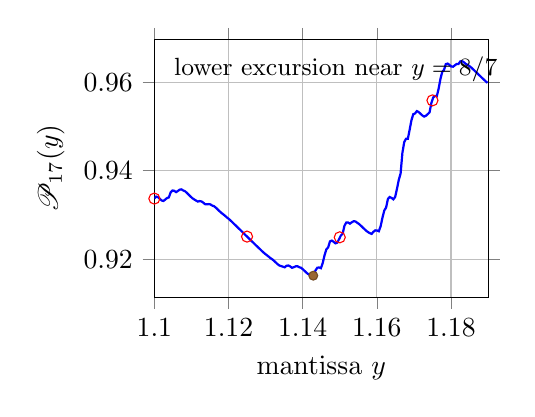
\begin{tikzpicture}
\begin{axis}[
 width=0.48\textwidth,
 height=0.40\textwidth,
 xlabel={mantissa $y$},
 ylabel={$\mathscr P_{17}(y)$},
 xmin=1.10,xmax=1.19,
 grid=major,
 tick align=outside,
 title={\small lower excursion near $y=8/7$},
 every axis title/.style={below right,at={(0.03,0.97)}},
]
\addplot+[mark=none,thick] coordinates {
(1.099998,0.9337475) (1.100487,0.9341566) (1.100975,0.9340251) (1.101463,0.9336773)
(1.101952,0.9332846) (1.102440,0.9331751) (1.102928,0.9334776) (1.103416,0.9338282)
(1.103905,0.9339770) (1.104393,0.9351113) (1.104881,0.9355436) (1.105370,0.9354617)
(1.105858,0.9351683) (1.106346,0.9354367) (1.106834,0.9357246) (1.107323,0.9357865)
(1.107811,0.9355241) (1.108299,0.9353521) (1.108788,0.9349841) (1.109276,0.9345783)
(1.109764,0.9341682) (1.110252,0.9337907) (1.110741,0.9335098) (1.111229,0.9332710)
(1.111717,0.9330283) (1.112206,0.9331395) (1.112694,0.9330624) (1.113182,0.9327950)
(1.113670,0.9324470) (1.114159,0.9324183) (1.114647,0.9324596) (1.115135,0.9323895)
(1.115623,0.9321180) (1.116112,0.9319736) (1.116600,0.9316400) (1.117088,0.9312481)
(1.117577,0.9308448) (1.118065,0.9304827) (1.118553,0.9301595) (1.119041,0.9298291)
(1.119530,0.9294640) (1.120018,0.9291505) (1.120506,0.9287823) (1.120995,0.9283894)
(1.121483,0.9279877) (1.121971,0.9275945) (1.122459,0.9271975) (1.122948,0.9267973)
(1.123436,0.9263949) (1.123924,0.9259927) (1.124413,0.9255906) (1.124901,0.9251889)
(1.125389,0.9247875) (1.125877,0.9243864) (1.126366,0.9239858) (1.126854,0.9235860)
(1.127342,0.9231874) (1.127831,0.9227955) (1.128319,0.9224057) (1.128807,0.9220125)
(1.129295,0.9216188) (1.129784,0.9212633) (1.130272,0.9209442) (1.130760,0.9206247)
(1.131248,0.9202789) (1.131737,0.9200110) (1.132225,0.9196672) (1.132713,0.9192845)
(1.133202,0.9188938) (1.133690,0.9185863) (1.134178,0.9184309) (1.134666,0.9183170)
(1.135155,0.9181660) (1.135643,0.9185076) (1.136131,0.9185713) (1.136620,0.9183710)
(1.137108,0.9180595) (1.137596,0.9181781) (1.138084,0.9183784) (1.138573,0.9184192)
(1.139061,0.9181841) (1.139549,0.9180645) (1.140038,0.9177274) (1.140526,0.9173423)
(1.141014,0.9169515) (1.141502,0.9166180) (1.141991,0.9164810) (1.142479,0.9164533)
(1.142967,0.9164699) (1.143456,0.9174579) (1.143944,0.9180588) (1.144432,0.9181237)
(1.144920,0.9179639) (1.145409,0.9191470) (1.145897,0.9208759) (1.146385,0.9222228)
(1.146873,0.9226601) (1.147362,0.9240262) (1.147850,0.9242044) (1.148338,0.9239411)
(1.148827,0.9235865) (1.149315,0.9237242) (1.149803,0.9245141) (1.150291,0.9253366)
(1.150780,0.9257738) (1.151268,0.9275645) (1.151756,0.9282794) (1.152245,0.9282992)
(1.152733,0.9280373) (1.153221,0.9283364) (1.153709,0.9285656) (1.154198,0.9285514)
(1.154686,0.9282505) (1.155174,0.9279784) (1.155663,0.9276003) (1.156151,0.9272097)
(1.156639,0.9268185) (1.157127,0.9264388) (1.157616,0.9261305) (1.158104,0.9258878)
(1.158592,0.9257205) (1.159081,0.9261889) (1.159569,0.9265223) (1.160057,0.9264939)
(1.160545,0.9263184) (1.161034,0.9274894) (1.161522,0.9294044) (1.162010,0.9310137)
(1.162498,0.9316751) (1.162987,0.9336317) (1.163475,0.9340610) (1.163963,0.9338637)
(1.164452,0.9335356) (1.164940,0.9340734) (1.165428,0.9359128) (1.165916,0.9379333)
(1.166405,0.9393593) (1.166893,0.9440472) (1.167381,0.9464890) (1.167870,0.9472202)
(1.168358,0.9472437) (1.168846,0.9492722) (1.169334,0.9514288) (1.169823,0.9527883)
(1.170311,0.9529632) (1.170799,0.9534978) (1.171288,0.9532752) (1.171776,0.9529012)
(1.172264,0.9525090) (1.172752,0.9522562) (1.173241,0.9524347) (1.173729,0.9528147)
(1.174217,0.9532057) (1.174706,0.9553197) (1.175194,0.9565824) (1.175682,0.9569099)
(1.176170,0.9568409) (1.176659,0.9585455) (1.177147,0.9607436) (1.177635,0.9623549)
(1.178123,0.9628160) (1.178612,0.9641314) (1.179100,0.9642394) (1.179588,0.9639491)
(1.180077,0.9635780) (1.180565,0.9635383) (1.181053,0.9638602) (1.181541,0.9641495)
(1.182030,0.9641580) (1.182518,0.9647422) (1.183006,0.9647790) (1.183495,0.9645293)
(1.183983,0.9641695) (1.184471,0.9639489) (1.184959,0.9636812) (1.185448,0.9633519)
(1.185936,0.9629668) (1.186424,0.9625822) (1.186913,0.9621870) (1.187401,0.9617914)
(1.187889,0.9613961) (1.188377,0.9610016) (1.188866,0.9606138) (1.189354,0.9602350)
(1.189842,0.9598731)
};
\addplot+[only marks,mark=o] coordinates {
(1.100,0.933706) (1.125,0.925107) (1.150,0.924945) (1.175,0.955916)
};
\addplot+[only marks,mark=*,mark size=1.6pt] coordinates {
(1.1428571,0.9162696)
};
\end{axis}
\end{tikzpicture}\hfill
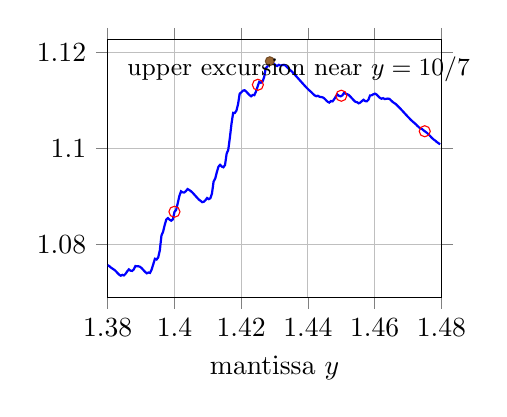
\begin{tikzpicture}
\begin{axis}[
 width=0.48\textwidth,
 height=0.40\textwidth,
 xlabel={mantissa $y$},
 xmin=1.38,xmax=1.48,
 grid=major,
 tick align=outside,
 title={\small upper excursion near $y=10/7$},
 every axis title/.style={below right,at={(0.03,0.97)}},
]
\addplot+[mark=none,thick] coordinates {
(1.379997,1.0757239) (1.380486,1.0755276) (1.380974,1.0752209) (1.381462,1.0749992)
(1.381950,1.0747767) (1.382439,1.0744839) (1.382927,1.0741106) (1.383415,1.0737672)
(1.383904,1.0735392) (1.384392,1.0737086) (1.384880,1.0735874) (1.385368,1.0739449)
(1.385857,1.0744518) (1.386345,1.0748496) (1.386833,1.0745818) (1.387321,1.0745276)
(1.387810,1.0748263) (1.388298,1.0755455) (1.388786,1.0754859) (1.389275,1.0754839)
(1.389763,1.0753621) (1.390251,1.0750527) (1.390739,1.0746772) (1.391228,1.0743146)
(1.391716,1.0740349) (1.392204,1.0741931) (1.392693,1.0741185) (1.393181,1.0748447)
(1.393669,1.0759401) (1.394157,1.0770461) (1.394646,1.0769003) (1.395134,1.0773322)
(1.395622,1.0787954) (1.396111,1.0819008) (1.396599,1.0826675) (1.397087,1.0840869)
(1.397575,1.0852296) (1.398064,1.0855208) (1.398552,1.0851820) (1.399040,1.0849764)
(1.399529,1.0852463) (1.400017,1.0867992) (1.400505,1.0872135) (1.400993,1.0886151)
(1.401482,1.0901148) (1.401970,1.0910816) (1.402458,1.0908676) (1.402946,1.0908484)
(1.403435,1.0911184) (1.403923,1.0915517) (1.404411,1.0913650) (1.404900,1.0911356)
(1.405388,1.0908326) (1.405876,1.0904648) (1.406364,1.0900863) (1.406853,1.0897095)
(1.407341,1.0893474) (1.407829,1.0891082) (1.408318,1.0888271) (1.408806,1.0889176)
(1.409294,1.0892429) (1.409782,1.0896875) (1.410271,1.0894504) (1.410759,1.0896431)
(1.411247,1.0906437) (1.411736,1.0931206) (1.412224,1.0937367) (1.412712,1.0950760)
(1.413200,1.0962251) (1.413689,1.0965691) (1.414177,1.0962361) (1.414665,1.0960758)
(1.415154,1.0965509) (1.415642,1.0989096) (1.416130,1.0997153) (1.416618,1.1022772)
(1.417107,1.1051866) (1.417595,1.1073975) (1.418083,1.1073596) (1.418571,1.1078564)
(1.419060,1.1092006) (1.419548,1.1113609) (1.420036,1.1116700) (1.420525,1.1120189)
(1.421013,1.1121058) (1.421501,1.1118385) (1.421989,1.1114598) (1.422478,1.1110985)
(1.422966,1.1108451) (1.423454,1.1111115) (1.423943,1.1110762) (1.424431,1.1118325)
(1.424919,1.1128879) (1.425407,1.1138369) (1.425896,1.1136510) (1.426384,1.1138785)
(1.426872,1.1148099) (1.427361,1.1167035) (1.427849,1.1170251) (1.428337,1.1176330)
(1.428825,1.1180390) (1.429314,1.1179736) (1.429802,1.1176095) (1.430290,1.1172938)
(1.430779,1.1171444) (1.431267,1.1173830) (1.431755,1.1172374) (1.432243,1.1173125)
(1.432732,1.1173736) (1.433220,1.1172691) (1.433708,1.1169192) (1.434196,1.1165922)
(1.434685,1.1162976) (1.435173,1.1160043) (1.435661,1.1156420) (1.436150,1.1152720)
(1.436638,1.1148966) (1.437126,1.1145181) (1.437614,1.1141396) (1.438103,1.1137613)
(1.438591,1.1133838) (1.439079,1.1130125) (1.439568,1.1126407) (1.440056,1.1123007)
(1.440544,1.1119872) (1.441032,1.1116977) (1.441521,1.1113375) (1.442009,1.1110395)
(1.442497,1.1108653) (1.442986,1.1109484) (1.443474,1.1107420) (1.443962,1.1106874)
(1.444450,1.1106109) (1.444939,1.1103862) (1.445427,1.1100210) (1.445915,1.1096976)
(1.446404,1.1095305) (1.446892,1.1098546) (1.447380,1.1097922) (1.447868,1.1102355)
(1.448357,1.1108014) (1.448845,1.1111982) (1.449333,1.1109288) (1.449821,1.1108370)
(1.450310,1.1110306) (1.450798,1.1115228) (1.451286,1.1113901) (1.451775,1.1112820)
(1.452263,1.1110827) (1.452751,1.1107532) (1.453239,1.1103812) (1.453728,1.1100166)
(1.454216,1.1096976) (1.454704,1.1096058) (1.455193,1.1093866) (1.455681,1.1095387)
(1.456169,1.1098433) (1.456657,1.1101193) (1.457146,1.1098449) (1.457634,1.1097917)
(1.458122,1.1101228) (1.458611,1.1110163) (1.459099,1.1110464) (1.459587,1.1112689)
(1.460075,1.1113840) (1.460564,1.1112168) (1.461052,1.1108573) (1.461540,1.1105336)
(1.462029,1.1103353) (1.462517,1.1104542) (1.463005,1.1102780) (1.463493,1.1103185)
(1.463982,1.1103677) (1.464470,1.1102837) (1.464958,1.1099477) (1.465446,1.1096470)
(1.465935,1.1093982) (1.466423,1.1091724) (1.466911,1.1088361) (1.467400,1.1084912)
(1.467888,1.1081343) (1.468376,1.1077674) (1.468864,1.1073992) (1.469353,1.1070314)
(1.469841,1.1066657) (1.470329,1.1063148) (1.470818,1.1059587) (1.471306,1.1056423)
(1.471794,1.1053489) (1.472282,1.1050635) (1.472771,1.1047104) (1.473259,1.1043943)
(1.473747,1.1041449) (1.474236,1.1040066) (1.474724,1.1037171) (1.475212,1.1034736)
(1.475700,1.1032125) (1.476189,1.1028938) (1.476677,1.1025319) (1.477165,1.1021796)
(1.477654,1.1018609) (1.478142,1.1016336) (1.478630,1.1013262) (1.479118,1.1010910)
(1.479607,1.1008645)
};
\addplot+[only marks,mark=o] coordinates {
(1.400,1.086830) (1.425,1.113237) (1.450,1.110962) (1.475,1.103570)
};
\addplot+[only marks,mark=*,mark size=1.6pt] coordinates {
(1.4285714,1.1181382)
};
\end{axis}
\end{tikzpicture}
\caption{The two narrow excursions of the Ces\`aro mantissa profile at
level $17$ (solid; boundary values at spacing $2^{-11}$), the first
audit's step-$0.025$ grid points (circles), and the exact values at
$y=8/7$ and $10/7$ (filled dots).  The $0.025$ grid interpolates
straight across both features --- the source of the first audit's
under-estimated range $[0.9249,1.1133]$ --- and even the $2^{-11}$
sampling does not reach the excursions' tips: the exact rational points
dip visibly beyond the sampled curve, as expected of a
singular-continuous limit profile.}
\label{fig:zoom}
\end{figure}

\subsection{The exact peak ray}
\label{ssec:peak-ray}

Document 6's identity
$|f(2^n\cdot\frac23)|=C_*E_{\kappa_\infty}(2^n\cdot\frac23)$, $n\ge0$,
was tested by direct 40-digit evaluation of the infinite product at
$n=0,5,10,15$: the four ratios agree with one another to
$2.8\cdot10^{-38}$, confirming exactness (not merely asymptotics), and
\[
 C_*=0.1391297747348293452945836\ldots,
\]
whose first fifteen digits are Document 6's print.  The identity
deserves emphasis because it is the cleanest possible witness that the
$\kappa_\infty$ envelope is attained: a single explicit geometric ray on
which the normalized transform is \emph{constant}.  It is also, with
the machinery already formalized, a near-term Lean target
(\cref{sec:lean}).

\section{Corrections to the first audit}
\label{sec:corrections}

For the record, the first audit's errors and imprecisions, as exposed
by the wave and verified here.  The companion patch updates the first
audit's text in place; this section is the changelog.

\begin{enumerate}
\item \textbf{``Unattainable in principle.''}  The first audit's
one-sentence summary called the unrestricted \eqref{eq:Q2}
``unattainable in principle.''  Its \emph{theorem} was correctly scoped
(stabilizing shapes only), and its verdict section stated the class
restriction --- but the slogan asserted more than was proved, and more
than is true: \cref{thm:adaptive} refutes it.  The corrected slogan:
unattainable for every gauge whose within-shell shape stabilizes or
stays within bounded distortion of the natural gauge --- attainable,
necessarily by unbounded shell-adaptive microstructure, in general.
\item \textbf{``Hardy-field (`elementary')''.}  The parenthetical
implied that Hardy-field covers all elementary formulas; Document 7's
oscillatory example $g_1\exp(\varepsilon\sin(c\log^2x))$ is elementary
and non-Hardy.  (It, too, fails \eqref{eq:Q2} --- by bounded
distortion --- so the first audit's conclusion survives for it; only
the implication arrow was wrong.)
\item \textbf{Profile range.}  $[0.9249,1.1133]$ was presented with a
grid caveat but used as ``the'' range; the true range contains
$[0.91627,1.11814]$ (\cref{ssec:profile-numerics}).
\item \textbf{$A_1^{\log}=0.0938610$.}  A seventh-significant-figure
error: the printed value was a finite-$K$ running mean of the shell
sequence $(\beta_k)$, whose $\bigO(1/K)$ Ces\`aro transient had not
died out.  Correct value $A_1^{\log}=0.09386063575678126\ldots$; the
first audit's own per-mantissa table ($0.093861$ at $y=1$) was already
consistent with it at its printed precision.
\item \textbf{$\kappa_1$ last digits.}  Shared with the whole corpus
(\cref{err:kappa1}).
\end{enumerate}

Nothing else in the first audit is contradicted by the wave: its
variance/LIL forensics, the singularity proof via
$\varrho_1\ge3^{-1/2}$, the logarithmic-mean theorem, the lobe-maxima
and RMS sections, and its per-document adjudications of Documents 1--4
all stand, and are independently re-derived in at least one second-wave
document each.

\section{Consequences for the corpus and the formalization ledger}
\label{sec:lean}

The repository's Lean formalization campaign
(\nolinkurl{Analysis/FabiusFunction/Lean/FabiusFunction/}) already
covers, in greater generality than the texts: the master lacunary
orthogonality theorem behind $\int_0^1P_n^2=2^{-n}$
(\lean{LacunaryRieszIntegral.lean}: \lean{integral_cos_mul_rieszProduct}
and its corollary \lean{integral_prod_sin_sq_two_pow}); the calibrated
Gelfond bound along \emph{every} logistic orbit and the resulting
$L^1$ lower bracket $\varrho_1\ge3^{-1/2}$
(\lean{GelfondLogisticBound.lean}: \lean{logistic_prod_le},
\lean{le_mul_integral_prod_abs_sin_two_pow}); and the dyadic shell
factorization with its exponent bookkeeping
(\lean{GeometricScaleProducts.lean}, \lean{SincProductShells.lean}:
\lean{norm_rvachevFourierProduct_two_pow_mul},
\lean{shell_exponent_identity}).  These are blocks 1 and 3 of
Document 8's proposed decomposition, plus the harder half of its
block 5.

The wave adds four attractive targets, in rough order of readiness:
\begin{enumerate}
\item \textbf{Sharp uniform bound} $\|P_n\|_\infty\le(\sqrt3/2)^{n-1}$
via the weighted two-step inequality (Documents 5/6) --- pure
trigonometric algebra plus a telescoping sum; same difficulty class as
the calibrated bound already formalized.
\item \textbf{The exact peak ray} $|f(2^n\cdot\frac23)|=
C_*E_{\kappa_\infty}(2^n\cdot\frac23)$ --- follows from
\lean{norm_rvachevFourierProduct_two_pow_mul} plus the exact
period-two orbit values $|\sin(2^j\cdot\frac{2\pi}3)|=\frac{\sqrt3}2$;
a satisfying exact statement with no analysis beyond the existing
modules.
\item \textbf{The martingale identity} $d=2\psi-\psi\circ\T=
\log|\tan\pi\cdot|$ with $\mathcal Pd=0$ (Document 6) --- pointwise
double-angle identities; the gateway to a formal variance computation.
\item \textbf{The flattening lemma} (Document 8's standalone form) ---
a measure-theoretic statement about weakly convergent measures,
independent of the sinc product; medium-term.
\end{enumerate}
The exact variance $\frac{\pi^2}4n-\frac{\pi^2}3(1-2^{-n})$ still
requires the Clausen expansion in $L^2$ and remains the hard
fluctuation target; the adaptive gauge's Hoischen step would enter as a
named classical import.

\subsection*{Postscript: ledger update (late August 2026 campaign)}

All four targets above are now formalized, and the campaign went
substantially further.  The development
(\nolinkurl{Analysis/FabiusFunction/Lean/FabiusFunction/}, seventy-one
sorry-free modules at this writing) now contains, kernel-checked:
\begin{itemize}
\item the sharp uniform bound $\|P_n\|_\infty\le(\sqrt3/2)^{n-1}$
with its full equality locus
(\lean{SharpGelfondBound}, \lean{SharpGelfondEquality});
\item the exact peak ray in product and $\kappa_\infty$-envelope form
(\lean{SincProductPeakRay}, \lean{PeakRayEnvelope});
\item the martingale identity $\mathcal Pd=0$ and the halving
$\mathcal P\psi=\psi/2$ (\lean{DoublingCocycleIdentities}), the full
Lasota--Yorke pair of the transfer operator with constants
$(\alpha,\beta,C)=(\sqrt2/4,\sqrt2/2,\pi/2)$
(\lean{TransferOperatorStep}) and its abstract Doeblin--Fortet
iteration and invariant ball (\lean{LasotaYorkeIteration});
\item \textbf{both Clausen values}:
$\int_0^1\log^2(2\sin\pi t)\,dt=\pi^2/12$ and
$\sigma^2=\int_0^1\log^2|\tan\pi t|\,dt=\pi^2/4$, obtained through the
Dirichlet-kernel cotangent pairing
(\lean{DirichletKernelCotangent}), the improper-integration-by-parts
evaluation of the log-sine Fourier coefficients $-1/(2m)$
(\lean{LogSineFourierCoefficient}), and interval Parseval with Basel
(\lean{CocycleParseval}, \lean{LogCosineFourier},
\lean{GordinParseval});
\item the complete covariance ladder $c_r=(\pi^2/12)\,2^{-r}$ for
\emph{every} lag over the genuine mod-one doubling map
(\lean{DoublingMapTransfer}, \lean{CovarianceLadder}), and the
martingale orthogonality of $d$ (\lean{MartingaleOrthogonality});
\item \textbf{the exact variance theorem itself}, stated on the
normalized dyadic sine product:
\[
  \int_0^1\log^2\Bigl|\prod_{k<n}2\sin(\pi 2^kt)\Bigr|\,dt
  =\frac{\pi^2}4\,n-\frac{\pi^2}3\bigl(1-2^{-n}\bigr)
\]
(\lean{DistanceCounting}, \lean{BirkhoffVariance},
\lean{BirkhoffProductBridge}) --- the finite-$n$ content of the
fluctuation theorem, fully numeric;
\item the flattening lemma's finite level (exact node equalization
and the partial-cell mesh bound, \lean{MeasureEqualization}) and its
diagonal selection mechanism (\lean{DiagonalSelection});
\item existence of the Perron root
$\varrho_1=\lim_n\|\mathcal L^n\mathbf 1\|_\infty^{1/n}
\in[1/2,\sqrt2/2]$ by Fekete's lemma
(\lean{TransferPositivity}, \lean{PerronRootExistence}), and its
uniqueness as an eigenvalue of positive continuous eigenfunctions by
the $m/M$-sandwich (\lean{PerronEigenvalueUnique}), together with the
exact centering $\int_0^1 S_n=0$ and the normalized limit
$(1/n)\int_0^1 S_n^2\to\pi^2/4$ (\lean{BirkhoffMoments});
\item \textbf{the one-peak theorem in full} (the drafts'
\texttt{thm:one-peak}): the log-factorization
$\log\lVert\Phi(x)\rVert=\sum_{(h,r)}\log\bigl(1-x^2/(2^h(r+1))^2\bigr)$
at every non-lattice real $x$, with the finitely many negative
factors absorbed by the $\log|\cdot|$ convention
(\lean{LobeLogFactorization}); strict concavity of $\log|\Phi|$ on
the central lobe $(-1,1)$ by twice-termwise differentiation of the
lattice log-series (\lean{CentralLobeConcavity},
\lean{CentralLobeOnePeak}); the peak pinned at the origin with
$\Phi(0)=1$ and $|\Phi(x)|<1$ on $(-1,1)\setminus\{0\}$, by evenness
and the strict midpoint inequality alone
(\lean{CentralLobePeakAtZero}); and strict concavity of
$\log\lVert\Phi\rVert$ on \emph{every} side lobe $\pm(m,m+1)$, via a
single uniform quadratic gap
$\min\bigl((u^2-m^2)/(m^2+1),\,1-v^2/(m+1)^2\bigr)\cdot a^2\le|a^2-y^2|$
powering both summable derivative majorants, plus the pointwise
interval glue (\lean{SideLobeConcavity}, \lean{OnePeakPerLobe}) ---
one peak per lobe, kernel-checked; moreover $\Phi$ is continuous on
the real axis (uniform products on compacts,
\lean{RvachevProductContinuity}), so each side lobe carries
\emph{exactly one} maximizer of $|\Phi|$ and the central maximizer is
exactly the origin;
\item \textbf{the unconditional fluctuation record}: exact centering
$\int_0^1\log|P_n|=0$, the $L^1$ scale
$\int_0^1|\log|P_n||\le(\pi/2)\sqrt n$ by the quadratic
Cauchy--Schwarz trick (\lean{LogProductMoments}); $\kappa_0=1$
\emph{in measure} --- for every $\varepsilon>0$,
$\operatorname{vol}\{t:|\log|P_n||\ge\varepsilon n\}
\le(\pi^2/4\varepsilon^2)/n\to0$ --- and the uniform-in-$n$
tightness $\operatorname{vol}\{t:|\log|P_n||\ge K\sqrt n\}
\le\pi^2/(4K^2)$ at the CLT scale, both by Chebyshev against the
exact variance (\lean{KappaZeroInMeasure},
\lean{FluctuationTightness}); and the baseline decay
$\|\Phi(x)\|\le1/(\pi|x|)$ on the whole real axis
(\lean{BaselineDecay});
\item \textbf{the zero order}: the dyadic lattice hits the integer
$m\ge1$ exactly $v_2(m)+1$ times (\lean{LatticeFiber}), and
$\|\Phi(x)\|/|x-m|^{\,v_2(m)+1}$ converges along the punctured
neighborhood of $m$ to an explicit strictly positive constant
(\lean{ZeroOrderTail}, \lean{PhiZeroOrder}) --- the multiplicity
statement of \texttt{prop:canonical} in quantitative local form, and
the local half of the valley law.  Its two extremes are corollaries:
$\Phi$ has \emph{simple} zeros at odd integers and zeros of order
$j+1$ at $2^j$, so the order is unbounded along the dyadic integers
(\lean{ValleyZeroOrders});
\item \textbf{the sign of $\Phi$, and it is Thue--Morse}: the split
product shows $\Phi$ is real on the whole real axis and, off the zero
lattice, $\Phi(x)=(-1)^{\#\{a\le|x|\}}\|\Phi(x)\|$
(\lean{PhiRealSign}); the exceptional block depends only on
$\lfloor\cdot\rfloor$, hence is constant along a lobe, and decomposes
into the fibers over $1,\dots,m$, giving one sign per lobe with
$\#\{a\le m\}=\sum_{k\le m}(v_2(k)+1)$ (\lean{LobeSignCount}).
Legendre's theorem in digit-sum form evaluates that count as
$2m-w(m)$, so
\[
  \Phi(x)=(-1)^{w(m)}\,\|\Phi(x)\|,\qquad x\in(m,m+1),
\]
with $w$ the binary digit sum (\lean{ThueMorseLobeSign}) --- the same
Thue--Morse sign that defines the signed global extension
$F=\sum(-1)^{w(n)}\,\mathrm{up}(\cdot-2n-1)$ governs the lobe signs of
its Fourier transform, and it is self-similar under doubling of the
frequency index (\lean{LobeSignSelfSimilarity});
\item \textbf{the renormalization identity} $\Phi(z)=\operatorname{sinc}(\pi z)\,\Phi(z/2)$
and its $n$-fold shell form (\lean{RenormalizationIdentity});
\item \textbf{the global $\kappa_\infty$ envelope}: there is a
constant $C$ with $\|\Phi(x)\|\le C\,E_{\kappa_\infty}(x)$ for every
$x\ge1$ (\lean{GlobalDecayEnvelope}).  The peak-ray gauge identity is
proved at an \emph{arbitrary} base point --- its $k$-linear terms
cancel precisely when $\kappa=\kappa_\infty$, so the identity
characterizes the exponent --- and is combined with the shell bound,
which already held along every dyadic ray, and a compact-window
maximum of $\|\Phi\|/E_{\kappa_\infty}$ on $[1,2]$.  With the
attainment along $2^k\cdot(2/3)$ this pins $\kappa_\infty$ from both
sides as \emph{the} envelope exponent of the Fourier decay;
\item the lacunary $L^1$ mean, sharpened from the Gelfond-inherited
$(\sqrt3/2)^n$ to $\int_0^1\prod_{j<n}|\sin(\pi2^jt)|\,dt\le2^{-n/2}$
by Cauchy--Schwarz against the exact second moment $2^{-n}$
(\lean{LacunaryMeanSharp}).
\end{itemize}
The sentence above about the exact variance is therefore superseded:
the Clausen expansion in $L^2$ is formalized, the one-peak profile
statement is now a theorem of the development rather than a target,
and of the fluctuation program only the limit theorems themselves
(the martingale central limit theorem and iterated-logarithm law),
the Rue\-lle--Perron--Frobenius eigenfunction \emph{existence}, and
the Hoischen approximation import remain outside the formalized
perimeter, all blocked on machinery currently absent from Mathlib.

\section{Verdict}
\label{sec:verdict}

\begin{enumerate}
\item \textbf{On the mathematics.}  The second wave completes the
problem.  The one genuinely open question --- unrestricted
\eqref{eq:Q2} --- is settled affirmatively by two independent, correct
constructions (Documents 7 and 8), and the impossibility side is
sharpened to bounded-distortion gauges (Document 7).  The final answer
to \cite{mse-decay} is the composite map of \cref{ssec:final-map}.
\item \textbf{On the documents.}  All four are of high quality and
essentially correct; their disagreements with one another are nil and
their corrections of the first audit are, in every case examined, fair.
Document 6 is the cleanest exposition of the fluctuation theory;
Document 7 carries the strongest new mathematics; Document 8
independently confirms it in a form best suited to formalization;
Document 5 is the most careful about scope and located the profile
features first.
\item \textbf{On the first audit.}  Its theorems all stand; its
numerics stand except one constant's seventh figure; two of its prose
claims were over-broad and are corrected here and, by patch, in place.
The episode is a textbook case for the repository's policy that
summary sentences must not outrun the theorems they summarize.
\item \textbf{On numerical hygiene.}  Three of the five errata found in
the wave are last-digit prints exceeding float64 pipeline precision.
The forty-digit values of \cref{ssec:constants} are now the corpus
reference; future documents should quote at most as many digits as
their own pipeline certifies.
\end{enumerate}

\appendix

\section{Reference constants after the second wave}
\label{app:constants}

Best current values, their sources, and status.  ``Proved'' means the
defining object is exact and the decimal is a stable high-precision
evaluation of it; only $\varrho_1$-derived quantities inherit the
caveat that $\varrho_1$ itself has a rigorous enclosure
($0.66130<\varrho_1<0.66135$ \cite{ahl2017}; Sturm certificate
$(0.66126807,0.66134891)$, Documents 4/6) much wider than its computed
precision.

\begin{center}
\small
\begin{tabular}{@{}lll@{}}
\toprule
constant & value & status \\
\midrule
$a=\log2$ & $0.69314718055994530942$ & exact \\
$\kappa_0$ & $3.15149612947231879805$ & exact ($\tfrac32+\log_2\pi$) \\
$\kappa_1$ & $2.74807001487133267392$ & from $\varrho_1$ (\cref{err:kappa1}) \\
$\kappa_2$ & $2.65149612947231879805$ & exact ($\log_22\pi$) \\
$\kappa_\infty$ & $2.35901487911174070735$ & exact ($\tfrac32+\log_2(\pi/\sqrt3)$) \\
$\varrho_1$ & $0.66132260206056561507352912$ & collocation, $N$-stable to $10^{-38}$ \\
$A_1$ & $0.09126612413158821228656$ & spectral $=$ direct to $16$ digits \\
$B_1$ & $0.06505923504037692143099$ & spectral $=$ direct to $16$ digits \\
$A_1^{\log}$ & $0.09386063575678126354068$ & $=B_1/a$ \\
$C_*$ & $0.13912977473482934529458$ & exact ray, $38$-digit constancy \\
$\beta=\log(\sqrt3/2)$ & $-0.14384103622589046372$ & exact \\
$c=(a/\pi)\sqrt{3/2}$ & $0.27022231973336534092$ & exact \\
$\varrho_2$ & $1/2$ & exact \\
$\varrho_3$ & $0.394896632370234$ & collocation \\
$\varrho_4$ & $0.320194101601104$ & collocation \\
$\varrho_8$ & $0.161244458899776$ & collocation \\
$\varrho_{16}$ & $0.050071935712638$ & collocation \\
$H(1)$ & $0.55377127588881009534$ & 30-digit product (first audit) \\
$\sigma^2$ per level & $\pi^2/4$ & proved (three routes) \\
LIL constant & $\pi/\sqrt2$ ($\sqrt{n\log\log n}$ norm.) & proved; published $\pi$ is the erratum \\
profile range & $\supseteq[0.91627,1.11814]$ & finite-level; extremes uncertified \\
\bottomrule
\end{tabular}
\end{center}

\section{Verification scripts}
\label{app:scripts}

\begin{itemize}
\item \nolinkurl{verification_scripts/stage7_spectral.py} ---
40-digit collocation: $\varrho_1$ ($N=48,64$), $A_1$, $B_1$,
$A_1^{\log}$, $C_*$ with the ray-constancy test, the $q$-spectrum,
Document 6's convergence table, Document 8's constants appendix,
$\Var(S_{1000})$, and $\int_0^{\pi/2}\log^2\tan=\pi^3/8$.  Writes
\nolinkurl{constants.json}.
\item \nolinkurl{verification_scripts/stage8_profile.py} ---
finite-level profile with integer-exact dyadic argument reduction:
direct $A_1^{(n)}$, $A_1^{\log(n)}$ for $n=13,\dots,20$; Document 5's
feature values by exact partial-cell quadrature; Document 7's
level-18/19 extremes; Document 6's sixteen-point table.
\item \nolinkurl{verification_scripts/stage8b_feature_zoom.py} ---
data for \cref{fig:zoom}.
\end{itemize}
All scripts were run on 26--27 August 2026; their complete output is
reproduced in the repository history alongside this file's commit.

\begin{thebibliography}{9}

\bibitem{mse-decay}
V.~Reshetnikov, \emph{Asymptotic decay rate of an infinite product of
sinc functions}, Mathematics Stack Exchange question 2745497 (2018);
repository transcription in
\nolinkurl{drafts/rvachev_up_fourier_decay/asymptotic-decay-rate-of-an-infinite-product-of-sinc-functions/}.

\bibitem{audit}
\emph{The Decay Envelope of the Rvachev Sinc Product: A Comparative
Audit}, second-wave report, this repository,
\nolinkurl{drafts/rvachev_up_fourier_decay/Rvachev_Up_Fourier_Decay_Comparative_Audit/}.

\bibitem{ahl2017}
C.~Aistleitner, R.~Hofer, G.~Larcher, \emph{On evil Kronecker sequences
and lacunary trigonometric products}, Ann.\ Inst.\ Fourier (Grenoble)
\textbf{67} (2017), no.~2, 637--687; local sources
\nolinkurl{docs/papers/arXiv-1502.06738v2/} and
\nolinkurl{docs/papers/AIF_2017__67_2_637_0/}.

\bibitem{ahl-corrected}
\emph{Corrected critical edition of the above},
\nolinkurl{docs/papers/AIF_2017__67_2_637_0/AIF_2017__67_2_637_0-corrected.tex}.

\bibitem{fm1996}
\'E.~Fouvry, C.~Mauduit, \emph{Sommes des chiffres et nombres presque
premiers}, Math.\ Ann.\ \textbf{305} (1996), 571--599.

\bibitem{hoischen}
L.~Hoischen, \emph{Eine Versch\"arfung eines Approximationssatzes von
Carleman}, J.\ Approx.\ Theory (1969/1975 series of papers on
approximation and interpolation by entire functions).

\bibitem{gauthier-kienzle}
P.~M.~Gauthier, J.~Kienzle, \emph{Approximation of a function and its
derivatives by entire functions}, Canad.\ Math.\ Bull.\ \textbf{59}
(2016), 87--94.

\bibitem{stout}
W.~F.~Stout, \emph{The Hartman--Wintner law of the iterated logarithm
for martingales}, Ann.\ Math.\ Statist.\ \textbf{41} (1970),
2158--2160; C.~C.~Heyde, D.~J.~Scott, Ann.\ Probab.\ \textbf{1} (1973),
428--436.

\bibitem{docs58}
Second-wave documents 5--8, this repository,
\nolinkurl{drafts/rvachev_up_fourier_decay/rvachev_up_fourier_decay-5} through
\nolinkurl{-8}.

\end{thebibliography}

\end{document}
